\documentclass{amsart}

\usepackage[english]{babel}
\usepackage{enumerate}
\usepackage{graphicx}

\title{The game of Risk analysed}
\author{Hidde Wieringa}
\date{\today}

\begin{document}
	
	\begin{abstract}
		In the game of Risk, the fights between two countries dominate the game. After explaining the rules of the game, these fights are examined rather closely. To do that, we need an optimal defend strategy, which will be used to calculate the worst case scenarios for the attacker. The possibilities of losing a certain number of units for the two opposing forces will be calculated. Because of these possibilities, it is possible to calculate the expected \emph{gain} in a certain state of the fight, as well as the probability for the attacker to win the fight.
	\end{abstract}
	
	\maketitle
	
	\section{The game of Risk}
	
	The game of Risk is played by three to six players. Each player gets assigned a number of areas on a world map, and gets an objective. Once a player has fulfilled this objective, the game ends. These objectives are either defeating another player, or conquering certain areas, usually in the form of continents. 
	
	To do that, a player will attack other players, in neighboring areas. A player can attack if he has more than one unit in the area. To attack, the attacker throws a minimum of one die, and a maximum of three dice. The defender then chooses whether he will defend with one or two dice. If the defender has only one unit, the player may only defend with one die. 
	
	Once the dice rolls are known, the maximum of each set is compared. If the attacker has a strict greater roll, the defender loses one unit. Else, the attacker loses one unit. This is repeated, until either the attacker or defender has rolled no more dice. 
	
	\section{The optimal defend strategy}
	
	The defender has the unique position be able to choose the amount of dice that will be used to defend the attacked area, after the attacker has rolled the attacking dice. This is a great advantage, because the defender can choose whether one or two armies must be put into the fight. Generally speaking, it is preferred to roll one die when the attacker rolled high, and two dice when the attacker rolled low. We will now make this strategy exact, to optimize the chances for the defender. 
	
	To do that, we first define the \emph{gain} of a defending roll as
	$$
		\text{gain}_A := E(G_A),
	$$ where $G$ is the stochastic value of the difference between the amount of attacking units destroyed and the amount of defending units lost, given the attacking roll $A$.
	
	Two find the optimal defending strategy, we look at each possible die roll for the three attacking dice. For two attacking dice we get the same results, as only the best two dice of the three count. When the attacker only rolls one die, it is always better for the defender to roll two dice when possible.
	
	We calculate the \emph{gain} for both strategies by calculating the mean gain when throwing with one die and when throwing with two dice. The results are shown in figure \ref{fig:1}. Only the two maximum dice are shown, as the minimum die does not influence the outcome of the fight. The chances of rolling such a roll for the attacker are also noted. 
	
	\begin{figure}
	
	\makebox[\textwidth]{
	\begin{tabular}{c||cc|cc|cc|cc|cc|cc}
	$A_1$ \,\textbackslash \, $A_2$ & \multicolumn{2}{c}{1} & \multicolumn{2}{c}{2} & \multicolumn{2}{c}{3} & \multicolumn{2}{c}{4} & \multicolumn{2}{c}{5} & \multicolumn{2}{c}{6} \\
	 & 1 & 2 & 1 & 2 & 1 & 2 & 1 & 2 & 1 & 2 & 1 & 2 \\ 
		
	\hline	
1 & 1.00 & 2.00 & & & & & & & & & &  \\ 
2 & 0.67 & 1.94 & 0.67 & 1.33 & & & & & & & &  \\ 
3 & 0.33 & 1.78 & 0.33 & 1.17 & 0.33 & 0.67 & & & & & &  \\ 
4 & 0.00 & 1.50 & 0.00 & 0.89 & 0.00 & 0.39 & 0.00 & 0.00 & & & &  \\ 
5 & -0.33 & 1.11 & -0.33 & 0.50 & -0.33 & 0.00 & -0.33 & -0.39 & -0.33 & -0.67 & &  \\ 
6 & -0.67 & 0.61 & -0.67 & 0.00 & -0.67 & -0.50 & -0.67 & -0.89 & -0.67 & -1.17 & -0.67 & -1.33  \\ 
	\end{tabular}
	}
	
	\vspace{10px}
	
	\makebox[\textwidth]{
	\begin{tabular}{c||cc|cc|cc|cc|cc|cc}
	$A_1$ \,\textbackslash \, $A_2$ & \multicolumn{2}{c}{1} &  \multicolumn{2}{c}{2} & \multicolumn{2}{c}{3} & \multicolumn{2}{c}{4} & \multicolumn{2}{c}{5} & \multicolumn{2}{c}{6} \\
		
	\hline	
1 & \textbullet\textbullet & 0.00  & & & & & & & & & &  \\ 
2 & \textbullet\textbullet & 0.01  & \textbullet\textbullet & 0.02  & & & & & & & &  \\ 
3 & \textbullet\textbullet & 0.01  & \textbullet\textbullet & 0.04  & \textbullet\textbullet & 0.03  & & & & & &  \\ 
4 & \textbullet\textbullet & 0.01  & \textbullet\textbullet & 0.04  & \textbullet\textbullet & 0.07  & \textbullet & 0.05  & & & &  \\ 
5 & \textbullet\textbullet & 0.01  & \textbullet\textbullet & 0.04  & \textbullet\textbullet & 0.07  & \textbullet & 0.10  & \textbullet & 0.06  & &  \\ 
6 & \textbullet\textbullet & 0.01  & \textbullet\textbullet & 0.04  & \textbullet\textbullet & 0.07  & \textbullet & 0.10  & \textbullet & 0.12  & \textbullet & 0.07   \\ 
	\end{tabular}
	}
	
	\caption{First table: the \emph{gain} when defending with either one or two dice. Second table: the optimal amount of dice to defend with, as well as the probability this situation occurs.} \label{fig:1}
	\end{figure}
	
	From this result we can conclude that the following simple rules (evaluated from the top) give us an optimal defending strategy, given attacking roll $A$ (sorted descending), attacking armies $X$ and defending armies $Y$:
	\begin{enumerate}
		\item If $Y = 1$, use one die,
		\item If $|A| = 1$, use two dice,
		\item If $A_2 > 3$, use one dice,
		\item Use two dice.
	\end{enumerate}
	
	We will use this set of rules to calculate the worst case scenario for the attacker concerning his chances of winning a fight. 
	
	\section{Destroyed units}
	
	Now that we have found an optimal defending strategy, let us look at the attacking force. When a force attacks, it can either lose one or two units, and the defender can also lose either one or two units in one roll for both parties. Depending on the dice rolls and the choices made, some of these chances of losing a certain number of units for both sides can be $0$. These events will be our event space 
	$$
	E = \{(2,0), (1,0), (1,1), (0,1), (0,2)\}.
	$$
	
	From now on we will assume the defender defends his area in an optimal way, to find a lower bound for the probabilities involved. 
	
	Much like the \emph{gain} which was calculated in the previous section, we will now calculate the probabilities of the different events which can take place after one roll of the attacker and defender. To do this, for each attacking roll each (optimal) defending row was calculated and the probability of those rolls occurring added to the probability of the event which occurs when those rolls are rolled. The results are listed in figure \ref{fig:2}. 
	
	\begin{figure}
	
	\makebox[\textwidth]{
	\begin{tabular}{c||ccccc}
		$X$ \,\textbackslash \, $Y$ & 1 & 2 & 3 & 4 \\
		\hline
		1 & \begin{tabular}{ll}
(0, 0) 1.00\end{tabular}& \begin{tabular}{ll}
(0, 0) 1.00\end{tabular}& \begin{tabular}{ll}
(0, 0) 1.00\end{tabular}& \begin{tabular}{ll}
(0, 0) 1.00\end{tabular} \\ \hline
2 & \begin{tabular}{ll}
(0, 1) 0.42\\(1, 0) 0.58\end{tabular}& \begin{tabular}{ll}
(0, 1) 0.25\\(1, 0) 0.75\end{tabular}& \begin{tabular}{ll}
(0, 1) 0.25\\(1, 0) 0.75\end{tabular}& \begin{tabular}{ll}
(0, 1) 0.25\\(1, 0) 0.75\end{tabular} \\ \hline
3 & \begin{tabular}{ll}
(0, 1) 0.58\\(1, 0) 0.42\end{tabular}& \begin{tabular}{ll}
(0, 1) 0.35\\(2, 0) 0.31\\(1, 0) 0.15\\(1, 1) 0.14\\(0, 2) 0.05\end{tabular}& \begin{tabular}{ll}
(0, 1) 0.35\\(2, 0) 0.31\\(1, 0) 0.15\\(1, 1) 0.14\\(0, 2) 0.05\end{tabular}& \begin{tabular}{ll}
(0, 1) 0.35\\(2, 0) 0.31\\(1, 0) 0.15\\(1, 1) 0.14\\(0, 2) 0.05\end{tabular} \\ \hline
4 & \begin{tabular}{ll}
(0, 1) 0.66\\(1, 0) 0.34\end{tabular}& \begin{tabular}{ll}
(0, 1) 0.37\\(2, 0) 0.20\\(1, 0) 0.13\\(1, 1) 0.17\\(0, 2) 0.14\end{tabular}& \begin{tabular}{ll}
(0, 1) 0.37\\(2, 0) 0.20\\(1, 0) 0.13\\(1, 1) 0.17\\(0, 2) 0.14\end{tabular}& \begin{tabular}{ll}
(0, 1) 0.37\\(2, 0) 0.20\\(1, 0) 0.13\\(1, 1) 0.17\\(0, 2) 0.14\end{tabular} \\
	\end{tabular}
	}
	
	\caption{For given $X$ and $Y$, the possible events $e \in E$ (the units destroyed for the attacker and defender) which can occur, with their respectible probabilities.} \label{fig:2}
	\end{figure}
	
	These probabilities are the same for any larger number of units on either side. Logical, since the attacking or defending strategy does not change when more units are added to either side.
	
	\section{Expected gain}
	
	As we have calculated the \emph{gain} for the defender in different scenarios, we will also calculate the gain for the attacker, given the attacking units $X$ and defending units $Y$. The plot of the gain is shown in figure \ref{fig:3}.
	
	\begin{figure}
	
	\makebox[\textwidth]{
	\begin{tabular}{c||ccccc}
		$X$ \,\textbackslash \, $Y$ & 1 & 2 & 3 & 4 & 5 \\
		\hline
		1 & 0.00 & 0.00 & 0.00 & 0.00 & 0.00  \\ 
		2 & -0.17 & -0.49 & -0.49 & -0.49 & -0.49  \\ 
		3 & 0.16 & -0.30 & -0.30 & -0.30 & -0.30  \\ 
		4 & 0.32 & 0.11 & 0.11 & 0.11 & 0.11  \\ 
		5 & 0.32 & 0.11 & 0.11 & 0.11 & 0.11  \\ 
	\end{tabular}
	}
	
	\caption{The gain of the attacker, given $X$ and $Y$ with the defender defending optimally.} \label{fig:3}
	\end{figure}
	
	\section{Winning probabilities}
	
	Finally we calculate the winning probabilities for the attacker, given the attacking units $X$ and defending units $Y$. Let $S = (X, Y)$ be the state of the fight. This state can change in any of the ways in the event set $E$. For any $e \in E$, there is a probability $P_{e,X,Y}$ that this event occurs. Once such an event occurs, the state changes to a new state, for which the same things can be said.
	
	This chain of events can be viewed as a Discrete Time Markov Chain, as no previous state influences the future of the current state. The chain will always enter an absorbing state which is of the form $(X, 0)$ or $(1, Y)$. These states are absorbing, because the attacker has won when the defender has no more units, and the defender wins once the attacker is left with one unit.
	
	To calculate the probability that the attacker wins, we set up the recurrence relation
	$$
	P_\text{win}(X, Y) = \sum_{e \in E} P_\text{win}(X - e_\text{att}, Y-e_\text{def}) \cdot P_{e, X, Y}, 
	$$
	using 
	$$
	P_\text{win}(X,0) = 1, P_\text{win}(1, Y) = 0
	$$
	for any $X$ and $Y$. The quantities $e_\text{att}$ and $e_\text{def}$ are the number of units that are destroyed of respectively the attacker and defender once event $e$ occurs.
	
	This recurrence relation can be solved recursively for any $X$ and $Y$, giving the results in figure \ref{fig:4}.
	
	\begin{figure}
	\makebox[\textwidth]{
	\begin{tabular}{c||cccccccccccccccc}
X \,\textbackslash \, Y &   0   &   1   &   2    &  3   &   4   &   5   &   6   &   7    &  8    &  9   &   10  &   11   &  12 &    13    & 14&     15  \\
\hline
1    &    - &   0.00 &   0.00 &   0.00 &   0.00 &   0.00 &   0.00 &   0.00 &   0.00 &   0.00 &   0.00 &   0.00 &   0.00 &   0.00 &   0.00 &   0.00 \\
2    &    1.00 &   0.42 &   0.11 &   0.03 &   0.01 &   0.00 &   0.00 &   0.00 &   0.00 &   0.00 &   0.00 &   0.00 &   0.00 &   0.00 &   0.00 &   0.00 \\ 
3    &    1.00 &   0.75 &   0.39 &   0.20 &   0.09 &   0.04 &   0.02 &   0.01 &   0.00 &   0.00 &   0.00 &   0.00 &   0.00 &   0.00 &   0.00 &   0.00 \\ 
4    &    1.00 &   0.92 &   0.67 &   0.47 &   0.31 &   0.20 &   0.12 &   0.08 &   0.05 &   0.03 &   0.02 &   0.01 &   0.01 &   0.00 &   0.00 &   0.00 \\ 
5    &    1.00 &   0.97 &   0.81 &   0.64 &   0.48 &   0.35 &   0.25 &   0.17 &   0.12 &   0.08 &   0.05 &   0.03 &   0.02 &   0.01 &   0.01 &   0.01 \\ 
6    &    1.00 &   0.99 &   0.90 &   0.78 &   0.64 &   0.51 &   0.39 &   0.29 &   0.21 &   0.15 &   0.11 &   0.08 &   0.05 &   0.04 &   0.02 &   0.02 \\ 
7    &    1.00 &   1.00 &   0.95 &   0.86 &   0.76 &   0.64 &   0.52 &   0.41 &   0.32 &   0.25 &   0.18 &   0.14 &   0.10 &   0.07 &   0.05 &   0.04 \\ 
8    &    1.00 &   1.00 &   0.97 &   0.92 &   0.84 &   0.74 &   0.64 &   0.53 &   0.44 &   0.35 &   0.27 &   0.21 &   0.16 &   0.12 &   0.09 &   0.07 \\ 
9    &    1.00 &   1.00 &   0.99 &   0.95 &   0.90 &   0.82 &   0.74 &   0.64 &   0.55 &   0.45 &   0.37 &   0.30 &   0.24 &   0.18 &   0.14 &   0.11 \\ 
10   &    1.00 &   1.00 &   0.99 &   0.97 &   0.94 &   0.88 &   0.81 &   0.73 &   0.64 &   0.56 &   0.47 &   0.39 &   0.32 &   0.26 &   0.20 &   0.16 \\ 
11   &    1.00 &   1.00 &   1.00 &   0.98 &   0.96 &   0.92 &   0.87 &   0.80 &   0.73 &   0.65 &   0.56 &   0.48 &   0.41 &   0.34 &   0.28 &   0.22 \\ 
12   &    1.00 &   1.00 &   1.00 &   0.99 &   0.98 &   0.95 &   0.91 &   0.86 &   0.80 &   0.73 &   0.65 &   0.57 &   0.50 &   0.42 &   0.36 &   0.30 \\ 
13   &    1.00 &   1.00 &   1.00 &   0.99 &   0.99 &   0.97 &   0.94 &   0.90 &   0.85 &   0.79 &   0.72 &   0.65 &   0.58 &   0.51 &   0.44 &   0.37 \\ 
14   &    1.00 &   1.00 &   1.00 &   1.00 &   0.99 &   0.98 &   0.96 &   0.93 &   0.89 &   0.84 &   0.79 &   0.72 &   0.66 &   0.59 &   0.52 &   0.45 \\ 
15   &    1.00 &   1.00 &   1.00 &   1.00 &   0.99 &   0.99 &   0.97 &   0.95 &   0.92 &   0.89 &   0.84 &   0.78 &   0.72 &   0.66 &   0.59 &   0.53 \\
	\end{tabular}}
	
	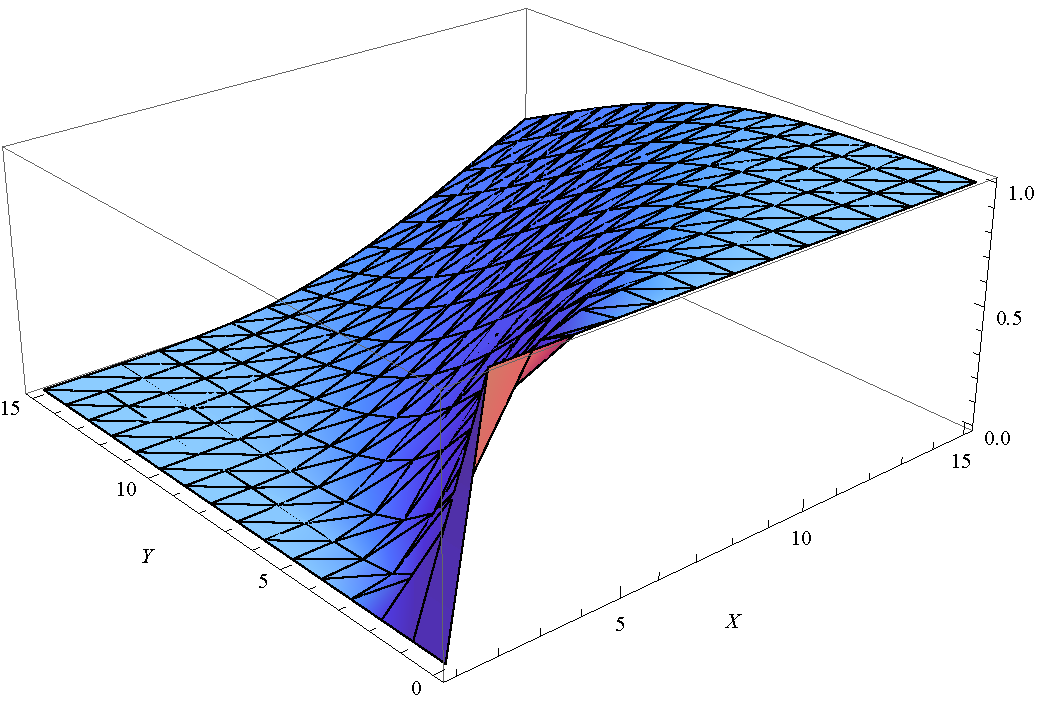
\includegraphics[scale=0.6]{Plot}
	
	\caption{The probability of winning a fight with $X$ attacking and $Y$ defending units, or $P_\text{win}(X,Y)$. Below that is a plot of the same data.} \label{fig:4}
	\end{figure}
	
	\section{conclusion}
	
	From the results of the last sections we can deduce two conclusions:
	\begin{enumerate}
		\item It is always better to have more units than your opponent. The more units you have while the opponents units stays the same amount, the more your winning probabilities increase.
	
		\item It is better for the attacker to save up units, even if the defender is doing the same. For equal $X$ and $Y$, the winning probabilities increase for larger $X$ and $Y$. 
	\end{enumerate}
	
	\section{Further ideas}
	
	This analysis is made solely for the game of Risk. Changing the rules of the game, any found results can be expanded easily. For example, one might change the number of states the dice can assume or the rules when and how many dice can be used to attack and defend. One can also create an more interesting problem by adding certain states in which units are added to the existing ones, instead of removed.
	
\end{document}